\part{Ejercicio 2}
\section{Enunciado}
La empresa Musimundo cuenta con una serie de sucursales repartidas por el pa'is. Recientemente ha decidido cerrar su sucursal
de Iruya y llevarse toda la mercader'ia al dep'osito central. Debido al dif'icil acceso ha dispuesto s'olo un cami'on para
llevar toda la mercader'ia. Sin embargo, es posible que no todo el material pueda ser llevado en un s'olo viaje del cami'on
d'ebido a las restricciones de carga, por lo que la parte que no entre en el cami'on ser'a vendida a valores despreciables el
 d'ia del cierre.

Dada la capacidad de carga m'axima P del cami'on y una lista de los productos del local conteniendo el valor $v_i$ y peso $p_i$ 
de cada uno, encontrar la lista de productos de mayor valor que sea posible llevar en el cami'on sin que el peso total de la
lista supere la carga m'axima. El valor de una lista de productos se calcula como la suma de los valores de los productos
involucrados. En caso de haber varias listas con el mismo valor m'aximo, encuentre cualquiera de ellas.
Realice un algoritmo para resolver el problema usando la t'ecnica de backtracking.

\section{Desarrollo}
\paragraph{}
Dado que el problema deb'ia ser resuelto con backtracking, buscamos la forma de aplicar dicha t'ecnica 
algor'itmica para su resoluci'on. B'asicamente la idea es formar todos los subconjuntos de cosas para 
encontrar aquel que maximice el valor total, sin exceder la capacidad de carga del cami'on.

\paragraph{}
A medida que se va armando una soluci'on, son descartadas aquellas cuyo peso excede la capacidad del 
cami'on, y de esta manera se va podando el 'arbol dejando solo posibles soluciones (por eso es 
backtracking y no fuerza bruta).

De esta manera, se construye el siguiente 'arbol de recursi'on:\\
\begin{figure}[H]
\centering
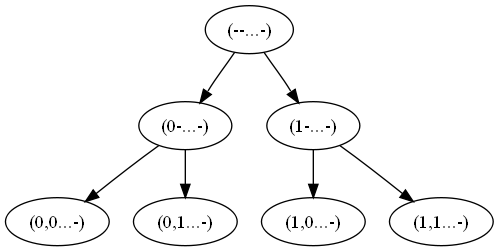
\includegraphics[scale=0.5]{./ejercicio2/arbol.png}
\end{figure}

\paragraph{}
En la ra'iz del 'arbol todavia no se determino para ningun elemento, si se lleva o no. Luego, en cada nodo se va construyendo una $n-upla$ donde un $0$ en la posici'on $i$ 
indica que el elemento $i$ no es parte de esta soluci'on, mientras que  un $1$ indica que el elemento est'a inclu'ido en la soluci'on.
Las hojas de este 'arbol son las soluciones posibles. Como cada elemento puede estar o no estar, se tienen dos posibilidades para cada
uno (llevarlo o no). Esto implica que la cantidad posible de soluciones si se tienen $n$ elementos es $2^n$.
\paragraph{}
El algoritmo implementado toma como par'ametros el cami'on (cosas, cuantas cosas y capacidad)  y dos soluciones posibles (una en donde est'a guardada la mejor 
encontrada hasta el momento y otra que guarda la que se va construyendo). Adem'as se lleva un 'indice que 
indica sobre que objeto se est'a decidiendo si conveniente o no llevarlo y el valor 'optimo que puede lograr una soluci'on
(se explica a continuaci'on).
\paragraph{}
B'asicamente una llamada a la funci'on consiste en verificar si se agrega o no a la soluci'on el elemento apuntado por $indice$. Si es as'i (es 
decir que al agregarlo, el peso total no excede el peso m'aximo), se agrega a la soluci'on candidata y se contin'ua con la 
siguiente llamada recursiva. Luego se realiza otra llamada recursiva que consiste en no agregar el elemento apuntado por 'indice. Cuando se encuentra 
una soluci'on mejor a la actualmente 'optima, 'esta es reemplazada. Repitiendo este proceso se pueden observar todas 
las hojas del 'arbol, para quedarse con la mejor.
\paragraph{}
Ademas de la restricci'on propia del problema, buscamos definir otras que nos permitieran efectuar mejores 
podas. Asi una primera idea fue ordenar el arreglo en orden creciente de pesos. De esta forma, si durante 
la construcci'on de una soluci'on, llegamos a que el elemento $k$ no se puede agregar, sabemos que ningun 
elemento entre $k+1$ y $n$ se va a poder agregar, porque su peso es mayor que el de $k$, y por ende mayor 
que la capacidad disponible.
\paragraph{}
Otra idea que tuvimos consisti'o en preguntar durante la contrucci'on de una soluci'on si tiene sentido 
que el algoritmo siga bajando por la rama que se deriva de este punto. Esto lo hacemos de la siguiente 
manera: si considero la suma de los valores de los elementos que me quedan por visitar y este valor 
sumado al del candidato actual no me da un valor m'as alto que el de la mejor soluc'ion hasta el momento, 
no tiene sentido que baje porque no voy a lograr una soluci'on con valor mayor. En un principio, para 
hacer esto se nos ocurri'o hacer la suma en cada llamada. Sin embargo este c'alculo era costoso, y por lo 
tanto buscamos alguna alternativa mejor. La idea entonces fue antes de empezar a trabajar con el arreglo 
de cosas, sumar el valor de todos los elementos. Este n'umero es el m'aximo valor que puedo lograr con 
un conjunto de cosas. Cada vez que hago una llamada calculo si el valor de mi candidato actual m'as el 
m'aximo me sirve para mejorar mi soluci'on. Por otro lado, cuando hago una llamada sin incluir a un 
elemento, resto al m'aximo posible el valor de dicho elemento.\\
\paragraph{}
Veamos un ejemplo: Tengo un conjunto de cosas tal que sus valores son: {1,2,3,4}. El m'aximo valor que podr'ia llevar 
es 10. Cuando estoy armando una soluci'on que excluye al valor 1, el m'aximo es 9. Si ademas quito al 2, 
el m'aximo es 7, etc. Consideramos que si bien estas podas no nos mejorar'ian el orden de complejidad, 
si nos permitir'ian en general observar un mejor desempe\~{n}o. Es importante notar que por como tenemos 
que devolver la soluci'on es necesario mapear de alguna manera los 'indices de los elementos luego de 
ordenarse con los del arreglo original. Esto agrega un \textsl{overhead} a la poda que debe tenerse en cuenta.
\paragraph{}
Para implementar el algoritmo se definieron los tipos $Cosa$, $Camion$ y $SolucionPosible$ con la finalidad de aportar m'as claridad al mismo.

\newpage
\section{Pseudoc'odigo}
\noindent
SolucionPosible: tupla$<cantCosas, guardo:[bool], valor, costo>$ \\
Camion: tupla$<cantCosas, capacidad, cosas: [Cosa]>$ \\
Cosa: tupla$<costo, valor>$ \\
cosas = $\{a_1,....,a_{cant}\}$ \\

\begin{algorithm}
\caption{Halla la soluci'on 'optima al problema del camion}
\begin{algorithmic}[1]
    \STATE s $\textcolor{orange}{\leftarrow}$ SolucionPosible\textcolor{magenta}{(}cant cosas\textcolor{magenta}{)}
    \STATE ordenar arreglo de cosas \COMMENT{mediante merge sort}
    \STATE valorMaximo $\textcolor{orange}{\leftarrow}$ $\sum_{t=0}^{cant cosas} \textcolor{magenta}{(}cosa_i\textcolor{magenta}{)}_{valor}$ 
    \STATE camionAux\textcolor{magenta}{(}s,c,0,mejorSol,valorMaximo\textcolor{magenta}{)}
\end{algorithmic}
\end{algorithm}

\begin{algorithm}
\caption{camionAux: Halla la solución óptima $mejorSol$ al problema del camion}
\begin{algorithmic}[1]
    \IF{ prob'e con las cant cosas \textcolor{orange}{\&} valor\textcolor{magenta}{(}candActual\textcolor{magenta}{)} $\textcolor{orange}{>}$ valor\textcolor{magenta}{(}mejorSol\textcolor{magenta}{)} }
        \STATE mejorSol $\textcolor{orange}{\leftarrow}$ candActual
        \STATE terminar
    \ENDIF    
    \IF{el valor del actual $\textcolor{orange}{+}$ valorMaximo $\textcolor{orange}{\leq}$ el valor de la mejor soluci'on hasta el momento}
        \STATE terminar
    \ELSE
        \IF {no prob'e las cant cosas}
                \IF {no me paso del peso máximo agregando $a_i$ a candActual}
                    \STATE agregar\textcolor{magenta}{(}$a_i$, candActual\textcolor{magenta}{)}
                    \STATE camionAux\textcolor{magenta}{(}candActual, cosas, capacidad, i\textcolor{orange}{+}1, cant, mejorSol\textcolor{magenta}{)}
                    \STATE sacar\textcolor{magenta}{(}$a_i$, candActual\textcolor{magenta}{)}
            		\ELSE
            								\STATE \COMMENT{ como los demas pesan mas, no puedo agregar a mas nadie}
		   	        						\IF{ valor\textcolor{magenta}{(}candActual\textcolor{magenta}{)} $\textcolor{orange}{>}$ valor\textcolor{magenta}{(}mejorSol\textcolor{magenta}{)} }
       											  	\STATE mejorSol $\textcolor{orange}{\leftarrow}$ candActual
        										\ENDIF	       
        										\STATE terminar
        				\ENDIF
         \STATE camionAux\textcolor{magenta}{(}candActual, cosas, capacidad, i\textcolor{orange}{+}1, cant, mejorSol\textcolor{magenta}{)}
    \ENDIF
   \ENDIF
\end{algorithmic}
\end{algorithm}

\paragraph{}
Por una cuesti'on de claridad (y para no desviar la atenci'on del algoritmo que realmente resuelve el problema), 
se excluy'o del pseudoc'odigo la traducci'on entre los 'indices originales, y los 'indices en que quedan los 
elementos luego de ordenarse (lo cual necesitamos para devolver la soluci'on en el formato pedido). Este proceso 
consiste en recorrer un diccionario (sobre arreglo) donde est'a mapeado para cada elemento la posici'on donde 
qued'o luego de ordenarse.
 
\newpage
\section{C'alculo de complejidad}
\paragraph{}
Para este ejercicio decidimos usar el modelo uniforme, ya que consideramos que lo que hace al n'ucleo del problema es la
cantidad de cosas a llevar. Por esa raz'on no nos parece desacertado considerar que el peso y el valor de las cosas estan 
acotados. Asimismo consideraremos que el tama\~{n}o de la entrada es la cantidad de cosas entre las cuales elegir 
(es decir la cantidad de items de la sucursal), en adelante $N$.
\paragraph{}
Antes de llamar a la funci'on que hace backtracking, el algoritmo ordena el arreglo con $merge sort$ en 
$O(N$ $log(N))$ y luego suma todos los valores del mismo en $O(N)$. Al finalizar el algoritmo, realizamos 
una traducci'on entre los indices originales de las cosas y su posici'on luego de ordenar que tiene un costo 
lineal, es decir $O(N)$. Veremos a continuaci'on que como el orden de la funci'on principal es mayor que 'estos, 
la complejidad total del algoritmo no se ve afectada.
\paragraph{}
Observemos que dado un $N$, si llamamos $n$ a la cantidad de elementos que quedan por procesar (es decir por 
decidir que hacer con ellos) se observa que $T(0) = N + 1$, pues hay que preguntar si encontr'e una 
mejor soluci'on y hay que copiar la soluci'on actual. Si no quedan m'as elementos que mirar y tengo que copiar 
la nueva soluci'on. Esta copia tiene como costo la cantidad de elementos entre los cuales hay que elegir.
\paragraph{}
Adem'as, si se observa el pseudoc'odigo, se puede ver que para un $n$ dado a lo sumo se hacen dos llamadas 
recursivas con $n - 1$ elementos a procesar. A este costo se le agrega una constante que llamaremos $k$, 
por lo tanto podemos deducir las siguientes ecuaciones de recurrencia:\\

$$T(0) = N + 1$$
$$T(n) = 2*T(n-1) + k$$

\paragraph{}
donde $k$ viene de las operaciones que se realizan dentro de cada llamada, que son todas $O(1)$.
\paragraph{}
En algun caso, podr'ia ocurrir que por accion de la poda, T(n) = N, ya que si la soluci'on que 
se est'a armando no puede incorporar ning'un objeto m'as (encontr'o que el elemento del 'indice actual 
es mayor al peso, y como est'an ordenados todos los siguientes pesan m'as) pero tiene un valor mayor 
que el de la mejor hasta el momento, hay que actualizar. Sin embargo, veremos a continuaci'on que en el 
caso donde esto no ocurre (el descripto por las ecuaciones) el orden es mayor que $N$.\\

Proponemos que: $$T(n) = N*2^n + k*(2^n-1) + 2^n$$

Lo podemos demostrar por inducci'on:\\

Para $n = 0$:\\

$$T(0) = N + 1 =  N*2^0 + k*(2^0-1) + 2^0$$

supongamos que vale para $n$, veamos que vale para $n+1$:

$$T(n+1) = 2T(n) + k$$

usando la hip'otesis inductiva:

$$T(n+1) = 2(N*2^n + k*(2^n-1) + 2^n) + k$$

$$T(n+1) = N*2^{n+1} + k*(2^{n+1}-2) + 2^{n+1} + k$$

$$T(n+1) = N*2^{n+1} + k*(2^{n+1}-1) + 2^{n+1}$$

Que era lo que quer'iamos ver.\\

Ahora bien como $T(n) = N*2^n + k*(2^n-1) + 2^n$ y adem'as sabemos que $n$ es del orden de $N$, tenemos que $T(n) \in$ $O(N*2^N)$.
\paragraph{}
Luego el algoritmo tiene un orden exponencial en funci'on del tama\~{n}o de la entrada, a'un pese a las podas; 
y esto es de esperarse ya que las podas funcionan 'unicamente en algunos casos, mientras que en otros no ayudan 
en nada. Otra forma de ver el orden es considerar el funcionamiento de algoritmo: la idea es revisar cada soluci'on 
posible, y sabemos que estas son $2^N$. En el peor de los casos, tenemos que recorrerlas todas y adem'as actualizar 
la mejor soluci'on cada vez. Como esto 'ultimo se realiza en a $O(N)$, el orden final del algoritmo resulta ser $O(2^N*N)$.
\paragraph{}
Si el algoritmo solo desecha un camino cuando no puede agregar a un elemento porque se excede del peso, el peor 
caso se da cuando puede poner a todos los elementos, ya que llegar'a a cada hoja. Observando las podas que implementamos, 
uno esperar'ia que en general el algoritmo se comporte bien, incluso en el caso antes mencionado. Ahora supongamos que 
tenemos un conjunto ${a_1,a_2,...a_N}$ donde el peso y el valor de $a_i = 1$ $\forall i \in {1...N-1}$ y el peso y valor de  
$a_N = N$ y que la capacidad del cami'on es $N$.
\paragraph{}
En este caso ninguna de nuestras podas va a funcionar, puesto que la poda por pesos baja siempre hasta el ante'ultimo nivel,
salvo en el caso donde no agregu'e a ning'un $a_i$ con $i < N$. Tampoco funciona ver cual es el m'aximo que puedo armar 
porque hasta que no llegue al caso donde solo pongo a $a_N$ el valor m'aximo que puedo armar siempre es mayor que $N$, 
pero las soluciones que arme siempre valen menos que $N$. Por ende en este caso se recorren pr'acticamente todas las ramas. 

\section{An'alisis experimental}
\subsection{Experiencias realizadas}
\paragraph{}
Para probar el comportamiento del algoritmo medimos tiempos y cantidad de operaciones en funci'on del tama\~{n}o de la 
entrada, es decir de la cantidad de posibles elementos a llevar. A modo de ver si nuestras podas representaban una mejora
en la pr'actica contrastamos los resultados entre el algoritmo sin podas, y el algoritmo con podas. 
\paragraph{}
Para hacer las pruebas generamos casos donde la cantidad de elementos era creciente y la composic'ion del conjunto de cosas era 
aleatoria. El peso que el cami'on puede cargar se fij'o en 200 y los valores y pesos de las cosas siguen una distribuci'on 
uniforme (0,100). Ademas se analiz'o el comportamiento del algoritmo en aquellas situaciones que consideramos como peores 
casos. En los gr'aficos, se denomina algoritmo sin poda a la versi'on que no ordena el arreglo, ni observa la suma potencial 
del camino.

\newpage
\subsection{Gr'aficos}

\begin{figure}[H]
\centering
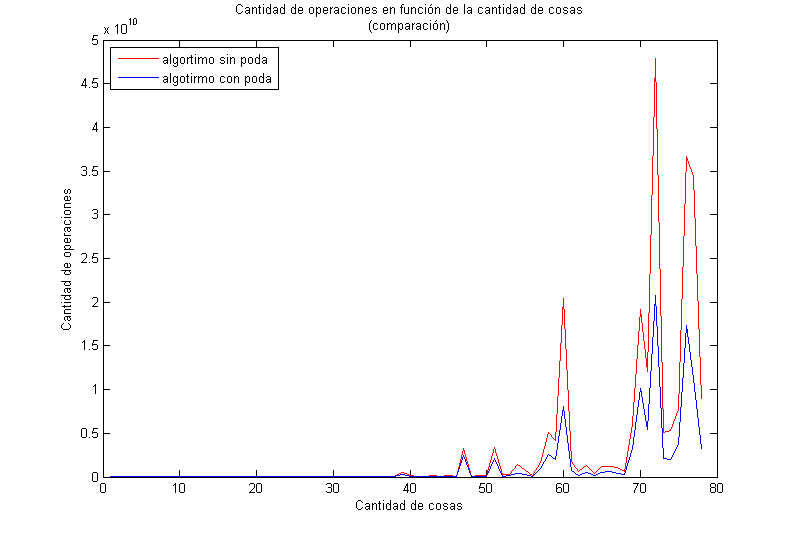
\includegraphics[scale=0.7]{../../codigo/ejercicio2/benchmark/graficos/comparacion_con_poda_sin_poda/caso_promedio/comparacionCantOpConPodaSinPoda.png}
\caption{Cantidad de operaciones en funci'on de la cantidad de cosas (peso y valor aleatorios con distribuci'on uniforme)}
\label{Ej2fig1}
\end{figure}

\begin{figure}[H]
\centering
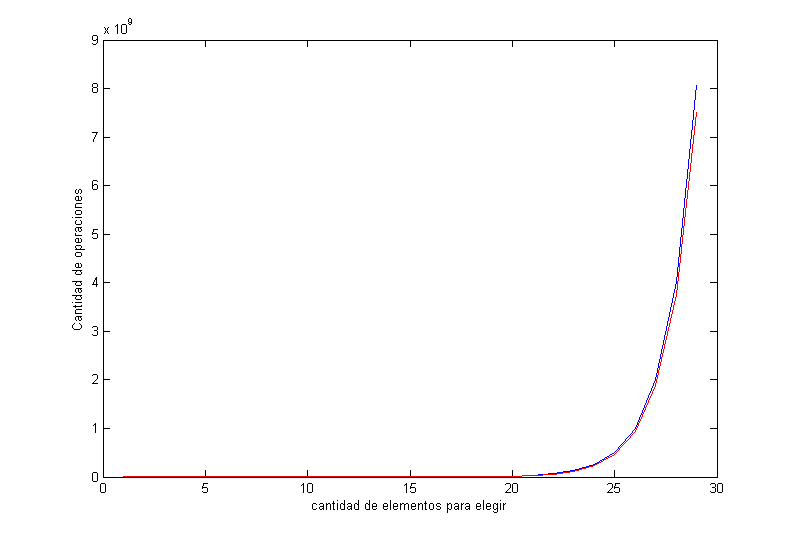
\includegraphics[scale=0.7]{../../codigo/ejercicio2/benchmark/graficos/operaciones_peor_caso_poda/peorCasoConPoda.png}
\caption{Cantidad de operaciones en funci'on de la cantidad de elementos, peor caso para la poda}
\label{Ej2fig2}
\end{figure}

\begin{figure}[H]
\centering
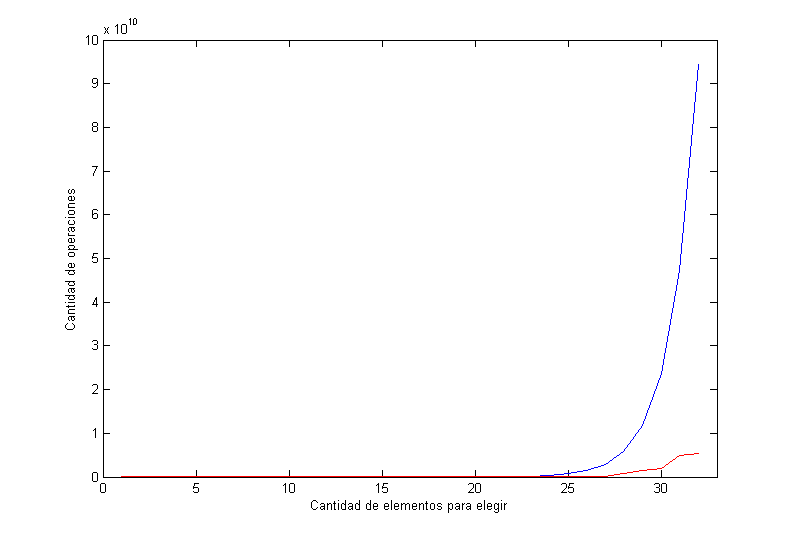
\includegraphics[scale=0.7]{../../codigo/ejercicio2/benchmark/graficos/operaciones_peor_caso_poda/peorCasoSinPoda.png}
\caption{Operaciones en funci'on de la cantidad de cosas, peor caso sin podas }
\label{Ej2fig3}
\end{figure}

\begin{figure}[H]
\centering
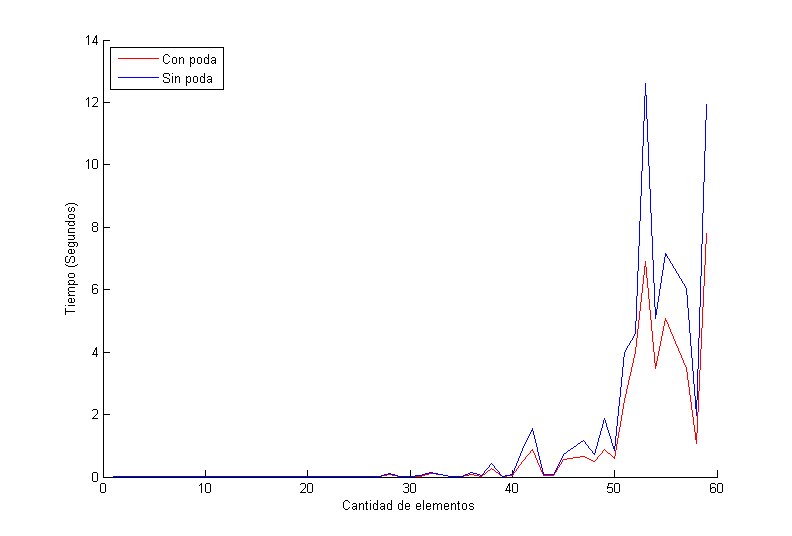
\includegraphics[scale=0.7]{../../codigo/ejercicio2/benchmark_tiempos/graficos/tiempo_caso_promedio/ComparacionPodavsSinPoda.png}
\caption{Tiempo en funci'on de la cantidad de cosas, casos aleatorios}
\label{Ej2fig4}
\end{figure}

\newpage
\section{Discusi'on}
\paragraph{}
En los gr'aficos pudimos observar el comportamiento exponencial del algoritmo. En las corridas de casos generales,
se observ'o un mejor comportamiento del algoritmo que implementaba las diversas podas, lo cual es esperable, puesto
que uno tender'ia a creer que algunas ramas se van a podar necesariamente si la configuraci'on de las cosas es aleatoria.
\paragraph{}
El algoritmo con podas se comport'o mucho mejor que el algoritmo sin podas en el peor caso de este 'ultimo: esto se 
explica porque en este caso la primer mejor soluci'on que se arma es la que es 'optima, y por eso no baja por ninguna 
rama, ya que ninguna tiene el potencial de superarla.
\paragraph{}
En el peor caso de nuestro algoritmo con podas s'i se observa que el comportamiento es peor que el del algoritmo 
com'un y esto se explica si tenemos en cuenta que en este caso no se hacen podas efectivas y sin embargo tenemos 
el \textsl{$overhead$} de ordenar el arreglo y hacer la traducci'on de los 'indices para poder reconstruir los valores que
se almacenan en el archivo de salida.
\paragraph{} 
El gr'afico de tiempos muestra la misma tendencia que el de cantidad de operaciones, y por tanto no merece
un an'alisis adicional.
\paragraph{} 
A modo de conclusi'on podemos decir que se validaron las hip'otesis planteadas durante el an'alisis te'orico.
